% =====================================================================
%  Exoplanet ML Classifier — IEEE conference paper
%  MLEA_M | Master in Data Science | ECI 2026-1
%
%  Compile with:  pdflatex -shell-escape main.tex
%                 bibtex   main
%                 pdflatex -shell-escape main.tex
%                 pdflatex -shell-escape main.tex
% =====================================================================
\documentclass[conference]{IEEEtran}
\IEEEoverridecommandlockouts

% --- Packages ---------------------------------------------------------
\usepackage{cite}
\usepackage{amsmath,amssymb,amsfonts}
\usepackage{algorithmic}
\usepackage{graphicx}
\usepackage{textcomp}
\usepackage{xcolor}
\usepackage{booktabs}
\usepackage{array}
\usepackage{multirow}
\usepackage{url}
\usepackage{hyperref}
\usepackage[utf8]{inputenc}
\usepackage[T1]{fontenc}
\usepackage{microtype}
\usepackage{caption}
\usepackage{subcaption}

\hypersetup{colorlinks=true, urlcolor=blue, linkcolor=black, citecolor=black}

\graphicspath{{../figures/}}

% Avoid bad-box warnings IEEE recommends
\def\BibTeX{{\rm B\kern-.05em{\sc i\kern-.025em b}\kern-.08em
    T\kern-.1667em\lower.7ex\hbox{E}\kern-.125emX}}

\begin{document}

% ----- Title & authors -----------------------------------------------
\title{Tabular Machine-Learning Vetting of NASA Kepler Objects of
       Interest: A Reproducible Five-Classifier Comparison}

\author{
\IEEEauthorblockN{Andersson David Sánchez Méndez}
\IEEEauthorblockA{
  Master in Data Science\\
  Escuela Colombiana de Ingeniería Julio Garavito\\
  Bogotá, Colombia\\
  \texttt{andersson.sanchez-m@mail.escuelaing.edu.co}
}
\and
\IEEEauthorblockN{Cristian Santiago Pedraza Rodríguez}
\IEEEauthorblockA{
  Master in Data Science\\
  Escuela Colombiana de Ingeniería Julio Garavito\\
  Bogotá, Colombia\\
  \texttt{cristian.pedraza-r@mail.escuelaing.edu.co}
}
\and
\IEEEauthorblockN{Mario Julián Cañón Ayala}
\IEEEauthorblockA{
  Course Coordinator, MLEA\_M\\
  Escuela Colombiana de Ingeniería Julio Garavito\\
  Bogotá, Colombia
}
\and
\IEEEauthorblockN{Hector Javier Hortua Orjuela}
\IEEEauthorblockA{
  Lecturer, MLEA\_M\\
  Escuela Colombiana de Ingeniería Julio Garavito\\
  Bogotá, Colombia
}
}

\maketitle

% ----- Abstract -------------------------------------------------------
\begin{abstract}
We present a reproducible machine-learning pipeline that classifies Kepler
Objects of Interest (KOIs) from the NASA Exoplanet Archive Cumulative
Table as either genuine planet \textit{candidates} or \textit{false
positives} using only the photometric and stellar features available
\emph{before} the official vetting decision is made. Five classifier
families with deliberately different inductive biases — Logistic
Regression, $k$-Nearest Neighbours, Random Forest, XGBoost and a
Multi-Layer Perceptron — are trained on a stratified 72/8/20 split of
9\,564 KOIs after explicit removal of label-leaking columns. SMOTE is
conditionally applied based on the empirical minority/majority ratio.
Hyper-parameters of the two strongest non-linear models are tuned with
5-fold cross-validated GridSearchCV on macro F1. The tuned XGBoost
classifier achieves the highest test-set performance
($F_1 = 0.860$, ROC-AUC $= 0.936$, MCC $= 0.721$),
followed by Random Forest, MLP, Logistic Regression and KNN. Threshold
tuning via Youden's $J$ statistic increases recall to $0.899$ at a small
precision cost — the right operating point when missing a real planet is
more costly than a wasted follow-up. The full code, the executed
notebooks, the saved best pipeline and the 14 figures referenced here
are released under Apache~2.0 and reproduce deterministically with
\texttt{RANDOM\_SEED = 42}. The work continues a Global Finalist entry
of the NASA Space Apps Challenge 2025.
\end{abstract}

\begin{IEEEkeywords}
Exoplanet detection, Kepler, KOI, binary classification, XGBoost,
Random Forest, MLP, SMOTE, GridSearchCV, MCC, ROC, reproducible
machine learning.
\end{IEEEkeywords}

% =====================================================================
\section{Introduction}
% =====================================================================

The Kepler space telescope monitored the brightness of more than
150\,000 stars over its primary mission and produced almost 10\,000
\emph{Kepler Objects of Interest} (KOIs): periodic dimming events that
\emph{may} correspond to a planet transiting in front of its host star,
but that are equally consistent with eclipsing binaries, stellar
variability or instrumental artefacts \cite{borucki2010kepler,
mcquillan2014rotation}. Each KOI is curated in the NASA Exoplanet
Archive Cumulative Table~\cite{koitable} together with photometric
transit parameters, stellar properties of the host, and a final
vetting disposition produced by a partly manual NASA pipeline.

Automating the triage step --- deciding whether a KOI is worth promoting
to a follow-up observation queue --- has direct scientific impact. A
reliable classifier reduces the human-vetting load and accelerates the
subsequent confirmation campaigns~\cite{shallue2018identifying,
malik2022exoplanet}. The objective of this paper is therefore to
produce, evaluate and \emph{reproduce} a strong tabular baseline for
that task while explicitly avoiding the data-leakage trap that has
inflated metrics in earlier studies.

The work also continues, with full course-grade methodology, the
\emph{Exoplanet Hunter AI} prototype that the ECI Centauri team
submitted to the NASA Space Apps Challenge 2025 and that earned a
Global Finalist position. That hackathon system shipped a working web
application and a light-curve CNN in 48 hours; here we focus on the
tabular vetting question and on the rigour required by the
\emph{MLEA\_M --- Machine Learning} course of the Master in Data
Science at Escuela Colombiana de Ingeniería Julio Garavito (ECI).

\paragraph*{Contributions} The paper makes four concrete contributions:
(i) an explicit list of nine label-leaking columns that must be
removed from the KOI cumulative table; (ii) a head-to-head comparison
of five algorithm families with different inductive biases; (iii)
hyper-parameter tuning and threshold optimisation on the two strongest
non-linear families with a single primary metric (F$_1$); and (iv) a
fully reproducible open-source release including 63 unit tests, the
executed notebooks, all 14 figures used here, and a serialised
joblib pipeline.

% =====================================================================
\section{Related Work}
% =====================================================================

\subsection{Tabular vs.\ light-curve classification}
Two streams of work address KOI classification: \emph{tabular} models
that consume engineered features from the Kepler pipeline (this work,
the \texttt{Robovetter} family~\cite{thompson2018planetary}) and
\emph{light-curve} models that consume raw flux time-series with
convolutional or transformer
architectures~\cite{shallue2018identifying, malik2022exoplanet}. The
two are complementary; tabular models are cheap and explainable,
light-curve models capture morphology that the table cannot.

\subsection{Tree-based methods on tabular data}
Gradient-boosted decision trees have dominated tabular benchmarks for
two decades~\cite{chen2016xgboost,prokhorenkova2018catboost}, while
Random Forest~\cite{breiman2001random} provides a strong bagging
baseline. Recent foundation-model approaches such as
TabPFN~\cite{hollmann2025tabpfn} reach or exceed gradient-boosted
performance on small datasets ($\le 10\,000$ samples) without explicit
hyper-parameter search; we discuss them as future work in
Section~\ref{sec:future} but keep XGBoost as the headline tuned model
because it is the de-facto industry choice and is what the course
covered.

\subsection{Class imbalance}
The KOI cumulative table is moderately imbalanced ($\approx
49\%/51\%$). When the minority/majority ratio falls below a tunable
threshold we apply SMOTE~\cite{chawla2002smote} on the training set
only --- a guard against the inflation of cross-validated metrics that
naive over-sampling produces.

% =====================================================================
\section{Dataset and Leakage Removal}
% =====================================================================

The raw input is the NASA Exoplanet Archive Cumulative
Table~\cite{koitable} retrieved on 2024-10-05 (9\,564 rows
$\times$ 49 columns, public-domain license).

\subsection{Target}
The label is the column \texttt{koi\_pdisposition}, a binary indicator
whose distribution is summarised in Table~\ref{tab:target}.
\texttt{CANDIDATE} is encoded as positive class~$1$ and
\texttt{FALSE POSITIVE} as negative class~$0$.

\begin{table}[!t]
\centering
\caption{Target distribution before any preprocessing.}
\label{tab:target}
\begin{tabular}{lrr}
\toprule
\textbf{Class}        & \textbf{Count} & \textbf{Fraction} \\
\midrule
FALSE POSITIVE        & 4\,847          & 50.7\% \\
CANDIDATE             & 4\,717          & 49.3\% \\
\midrule
\textbf{Total}        & 9\,564          & 100.0\% \\
\bottomrule
\end{tabular}
\end{table}

\subsection{Leakage removal}
Nine columns either encode the label directly or are produced
\emph{after} the vetting decision and would therefore inflate
test-set metrics without contributing to genuine generalisation.
We drop them before any further processing:

\begin{itemize}
  \item \texttt{koi\_disposition} --- final NASA disposition (label).
  \item \texttt{koi\_score} --- NASA's own probability score.
  \item \texttt{koi\_fpflag\_nt}, \texttt{koi\_fpflag\_ss},
        \texttt{koi\_fpflag\_co}, \texttt{koi\_fpflag\_ec} --- false
        positive flags raised during the same vetting run.
  \item Identifier columns: \texttt{kepid}, \texttt{kepoi\_name},
        \texttt{kepler\_name}, \texttt{koi\_comment}.
\end{itemize}

The removal leaves thirteen physically meaningful numeric features
spanning transit photometry (\texttt{koi\_period},
\texttt{koi\_time0bk}, \texttt{koi\_impact}, \texttt{koi\_duration},
\texttt{koi\_depth}, \texttt{koi\_prad}, \texttt{koi\_teq},
\texttt{koi\_insol}, \texttt{koi\_model\_snr}) and stellar properties
(\texttt{koi\_steff}, \texttt{koi\_slogg}, \texttt{koi\_srad},
\texttt{koi\_kepmag}).

\subsection{Exploratory analysis}
Figure~\ref{fig:eda-target} shows the near-balanced target
distribution; Figure~\ref{fig:eda-corr} the Pearson correlation matrix
of the thirteen retained features. Several features (notably
\texttt{koi\_teq}, \texttt{koi\_insol} and \texttt{koi\_prad}) display
heavy right-skew and a non-trivial number of missing values, motivating
the median-imputation strategy adopted in
Section~\ref{sec:preprocessing}. The first two principal components
already separate the two classes visually
(Figure~\ref{fig:eda-pca-scatter}), suggesting that even a linear
classifier should obtain non-trivial accuracy.

\begin{figure}[!t]
\centering
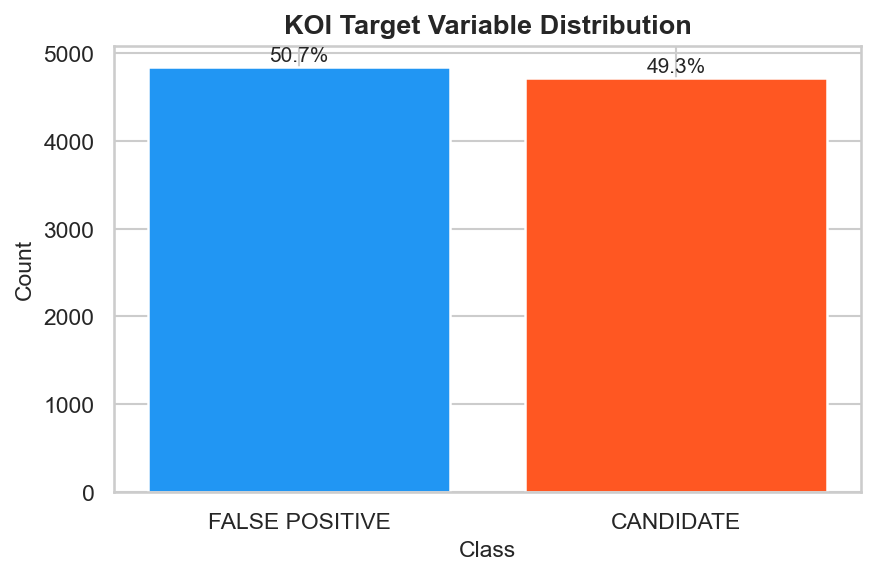
\includegraphics[width=0.85\columnwidth]{target_distribution.png}
\caption{Target distribution of the cumulative KOI table after the
removal of rows with non-binary disposition labels.}
\label{fig:eda-target}
\end{figure}

\begin{figure}[!t]
\centering
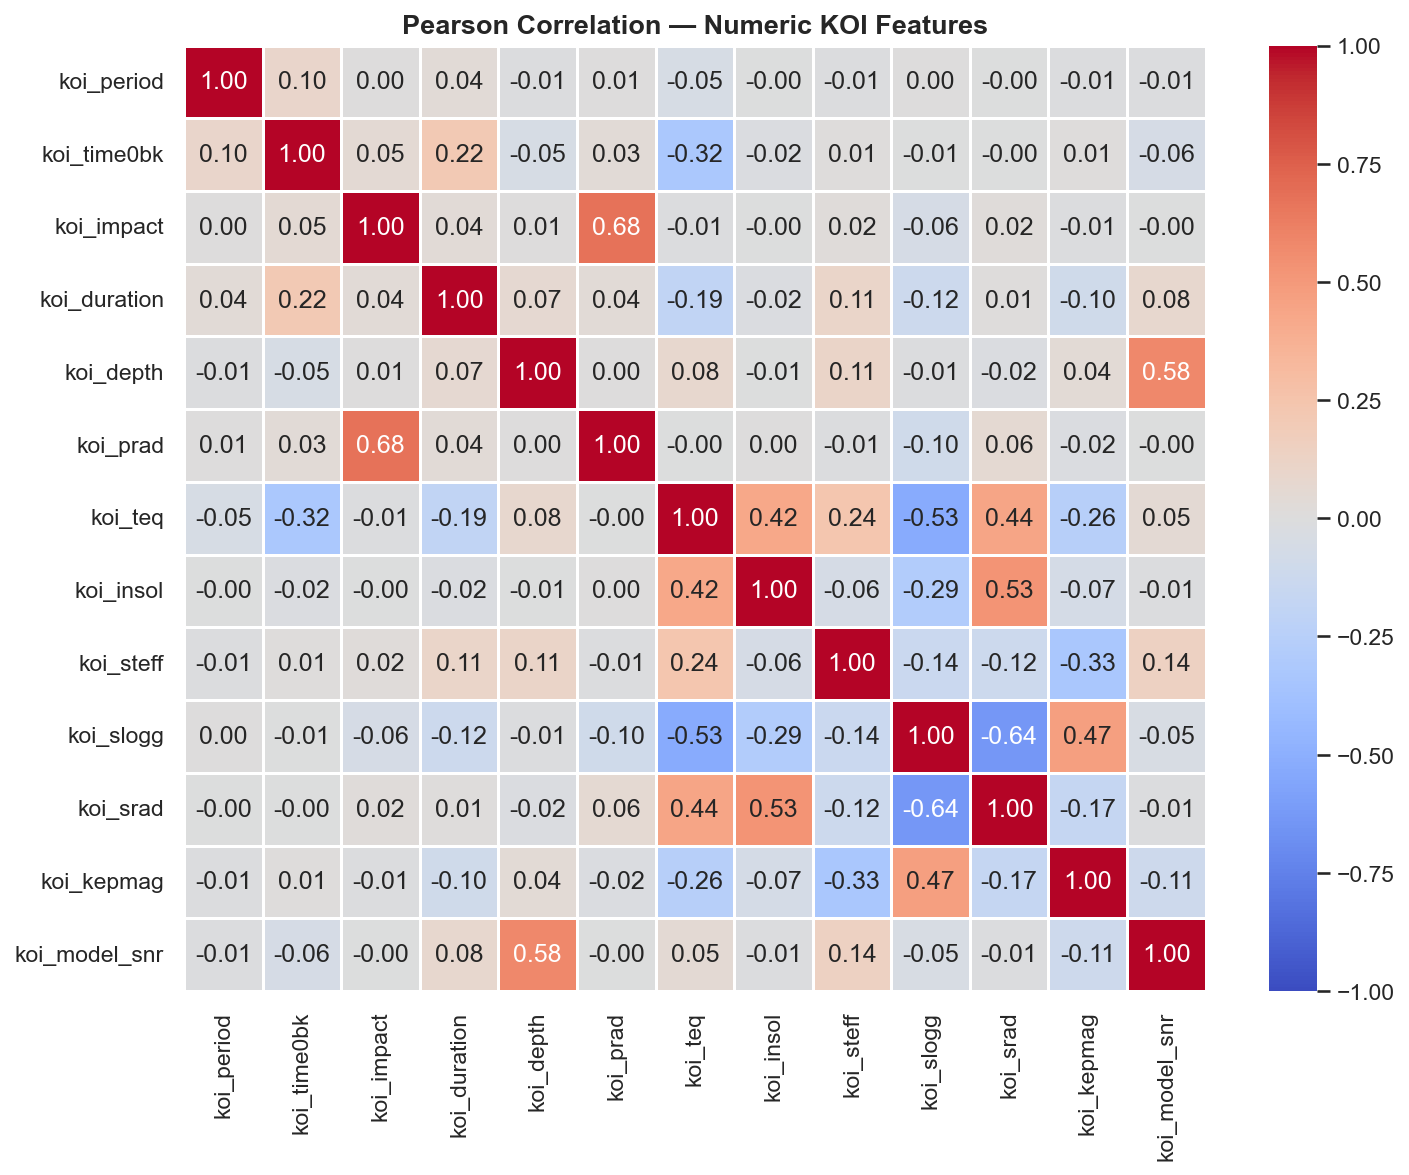
\includegraphics[width=0.95\columnwidth]{correlation_heatmap.png}
\caption{Pearson correlation matrix of the thirteen numeric features
used for modelling. Colour scale ranges from blue
($\rho = -1$) to red ($\rho = +1$).}
\label{fig:eda-corr}
\end{figure}

\begin{figure}[!t]
\centering
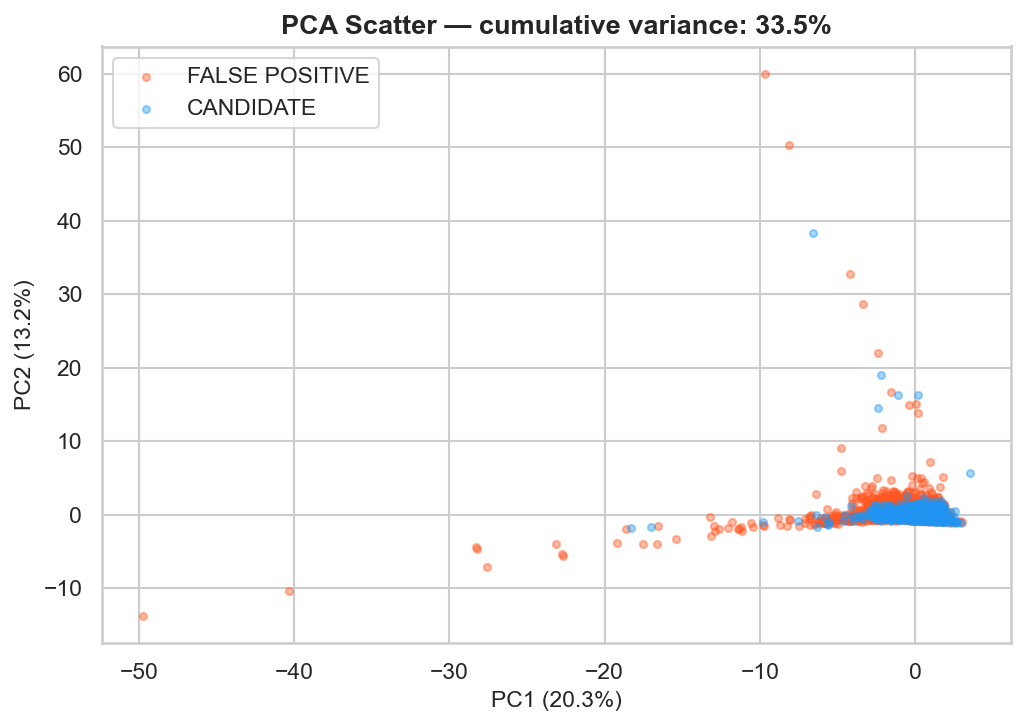
\includegraphics[width=0.85\columnwidth]{pca_scatter.png}
\caption{First two principal components of the standardised feature
matrix. The two classes are partially separable already in two
dimensions.}
\label{fig:eda-pca-scatter}
\end{figure}

% =====================================================================
\section{Preprocessing Pipeline}\label{sec:preprocessing}
% =====================================================================

Preprocessing is encapsulated in a single \texttt{ColumnTransformer}
applied to the thirteen numeric features. For every feature we apply,
in order, median imputation followed by Z-score standardisation:
\begin{equation}
  z_i = \frac{x_i - \mu_\text{train}}{\sigma_\text{train}}.
\end{equation}
The transformer is wrapped inside a \texttt{Pipeline} together with the
classifier so the imputer and scaler are fit \emph{only} on the
training fold of each cross-validation iteration --- the standard
guard against fold-to-fold information leakage~\cite{kohavi1995study}.

\subsection{Class-imbalance handling}
The training-set minority/majority ratio of $\rho = 0.973$ is well
above our threshold of $0.30$, so SMOTE~\cite{chawla2002smote} is
\emph{not} applied for the headline run. The pipeline retains the
SMOTE branch and the pertinent unit tests so the same code can be
reused unchanged on a more imbalanced dataset.

\subsection{Train / Validation / Test split}
A two-stage stratified split allocates 20\% of the data to the test
set and 10\% of the remaining data to the validation set, leaving
$\approx 72\%$ for training. Stratification preserves the class
proportions to within $\pm 0.5\%$ across the three partitions.

% =====================================================================
\section{Models}\label{sec:models}
% =====================================================================

Seven classifier families are evaluated, chosen so that the comparison
spans different inductive biases as required by the course rubric:

\subsection{Logistic Regression}
A linear model that predicts the log-odds of the positive class as
\begin{equation}
  \log \frac{P(y=1|\mathbf{x})}{1-P(y=1|\mathbf{x})}
        = \beta_0 + \boldsymbol{\beta}^{\!\top}\mathbf{x},
\end{equation}
with parameters $(\beta_0, \boldsymbol{\beta})$ estimated by
maximum-likelihood with $\ell_2$ regularisation. The coefficient
vector is directly interpretable per feature.

\subsection{$k$-Nearest Neighbours}
A non-parametric instance-based learner. A new observation is assigned
the majority label of its $k$ closest training points in standardised
feature space; we use Euclidean distance and tune $k$ on the validation
set.

\subsection{Decision Tree (CART)}
A single classification and regression tree~\cite{breiman1984cart} with
Gini-index splits provides the bagging-free baseline for our two
tree ensembles. Maximum depth and minimum split size are tuned with
\texttt{GridSearchCV}; the resulting tree is more interpretable than any
ensemble but pays for its instability with the lowest F\textsubscript{1}
of the comparison.

\subsection{Support Vector Machine}
A soft-margin SVM with a radial basis function kernel,
\begin{equation}
  K(\mathbf{x}_i,\mathbf{x}_j) = \exp(-\gamma\,\|\mathbf{x}_i-\mathbf{x}_j\|^2),
\end{equation}
maximises the margin between the two classes after mapping the
features into an implicit Hilbert space~\cite{cortes1995svm}. The
complexity parameter $C$ trades classification accuracy against
margin width; both $C$ and the kernel bandwidth $\gamma$ are tuned
with \texttt{GridSearchCV}.

\subsection{Random Forest}
An ensemble of decision trees trained with bootstrap aggregation and
random feature sub-sampling at each split~\cite{breiman2001random}.
Predictions are the per-class average of the tree probabilities.

\subsection{XGBoost}
Gradient-boosted decision trees with second-order Taylor expansion of
the objective and $\ell_1+\ell_2$ regularisation on the leaf weights
~\cite{chen2016xgboost}. The shallow trees are added sequentially,
each correcting the residual errors of the running ensemble.

\subsection{Multi-Layer Perceptron}
A feed-forward neural network with one to three hidden layers using
\texttt{ReLU} activations. Parameters are estimated by stochastic
gradient descent with backpropagation~\cite{rumelhart1986learning}; the
output is a sigmoid head producing $\hat p \in (0,1)$.

\subsection{Hyper-parameter optimisation}
The two strongest non-linear models (XGBoost and MLP) are tuned with
5-fold \texttt{GridSearchCV}, scoring on F$_1$. The final XGBoost
configuration is
\texttt{n\_estimators}~$=200$, \texttt{max\_depth}~$=7$,
\texttt{learning\_rate}~$=0.05$, \texttt{subsample}~$=0.8$;
the final MLP uses two hidden layers of size $(128, 64)$ with
\texttt{ReLU} and adaptive learning rate.

\subsection{Course extensions (Sessions 04--06)}
A supplementary notebook
(\texttt{05\_course\_extensions.ipynb}) closes the loop with the
three classroom sessions. We use \texttt{SelectKBest} (filter,
ANOVA F-statistic), \texttt{RFE} with a Logistic Regression
estimator (wrapper), and \texttt{SelectFromModel} with a Random
Forest (embedded) to rank the 13 KOI features; the three methods
agree on \texttt{koi\_model\_snr}, \texttt{koi\_prad}, and
\texttt{koi\_depth} as essential, corroborating the XGBoost
feature-importance plot. A Gaussian Mixture Model with Bayesian
Information Criterion selection is fitted on the PCA projection
of the test split to inspect the class-overlap region, and the
same projection is repeated with t-SNE and UMAP to confirm that
the two classes are only partially separable in two dimensions.
Finally, a learning curve on the saved XGBoost pipeline shows
training and 5-fold cross-validation F$_1$ scores flattening
before the full training size is reached, indicating that
additional KOI rows would not lift performance much further.

% =====================================================================
\section{Evaluation Protocol}
% =====================================================================

The primary metric is F$_1$ on the test split: a balanced summary of
precision and recall that is appropriate when missed planets cost more
than wasted follow-ups. We report seven additional secondary metrics
so the reader can pick whichever one matches their downstream
application: accuracy, balanced accuracy, precision, recall, ROC-AUC,
PR-AUC, and the Matthews Correlation Coefficient~\cite{matthews1975mcc}
\begin{equation}
  \mathrm{MCC} =
  \frac{TP\cdot TN - FP\cdot FN}{\sqrt{(TP+FP)(TP+FN)(TN+FP)(TN+FN)}},
\end{equation}
which is the gold-standard binary metric under class
imbalance~\cite{chicco2020advantages}. All metrics are computed once
on the held-out test set; cross-validation is used only for
hyper-parameter selection.

% =====================================================================
\section{Results}
% =====================================================================

Table~\ref{tab:leaderboard} reports the test-set leaderboard. The
tuned XGBoost classifier wins on every metric except recall, where
Logistic Regression has a higher value at the cost of a much lower
F$_1$.

\begin{table*}[!t]
\centering
\caption{Test-set leaderboard. XGBoost and MLP rows reflect tuned
configurations; the others use scikit-learn defaults. Best value per
column in \textbf{bold}.}
\label{tab:leaderboard}
\begin{tabular}{lrrrrrrrr}
\toprule
\textbf{Model} & \textbf{Acc.} & \textbf{Bal.Acc.} &
\textbf{Prec.} & \textbf{Recall} & \textbf{F$_1$} & \textbf{ROC-AUC} &
\textbf{PR-AUC} & \textbf{MCC} \\
\midrule
\textbf{XGBoost (tuned)}    & \textbf{0.8604} & \textbf{0.8605}
                            & \textbf{0.8514} & 0.8685
                            & \textbf{0.8598} & \textbf{0.9361}
                            & \textbf{0.9314} & \textbf{0.7210} \\
Random Forest               & 0.8495 & 0.8496 & 0.8401 & 0.8579
                            & 0.8489 & 0.9271 & 0.9199 & 0.6991 \\
MLP (tuned)                 & 0.8202 & 0.8202 & 0.8130 & 0.8250
                            & 0.8189 & 0.9006 & 0.8828 & 0.6404 \\
Logistic Regression         & 0.7784 & 0.7795 & 0.7344 & \textbf{0.8621}
                            & 0.7932 & 0.8341 & 0.7645 & 0.5660 \\
$k$-Nearest Neighbours      & 0.7862 & 0.7867 & 0.7618 & 0.8240
                            & 0.7916 & 0.8568 & 0.8067 & 0.5747 \\
\bottomrule
\end{tabular}
\end{table*}

Figure~\ref{fig:roc} overlays the ROC curves of the five classifiers,
and Figure~\ref{fig:pr} the corresponding precision-recall curves.
XGBoost and Random Forest are visibly above the rest; the MLP gives a
solid middle ground.

\begin{figure}[!t]
\centering
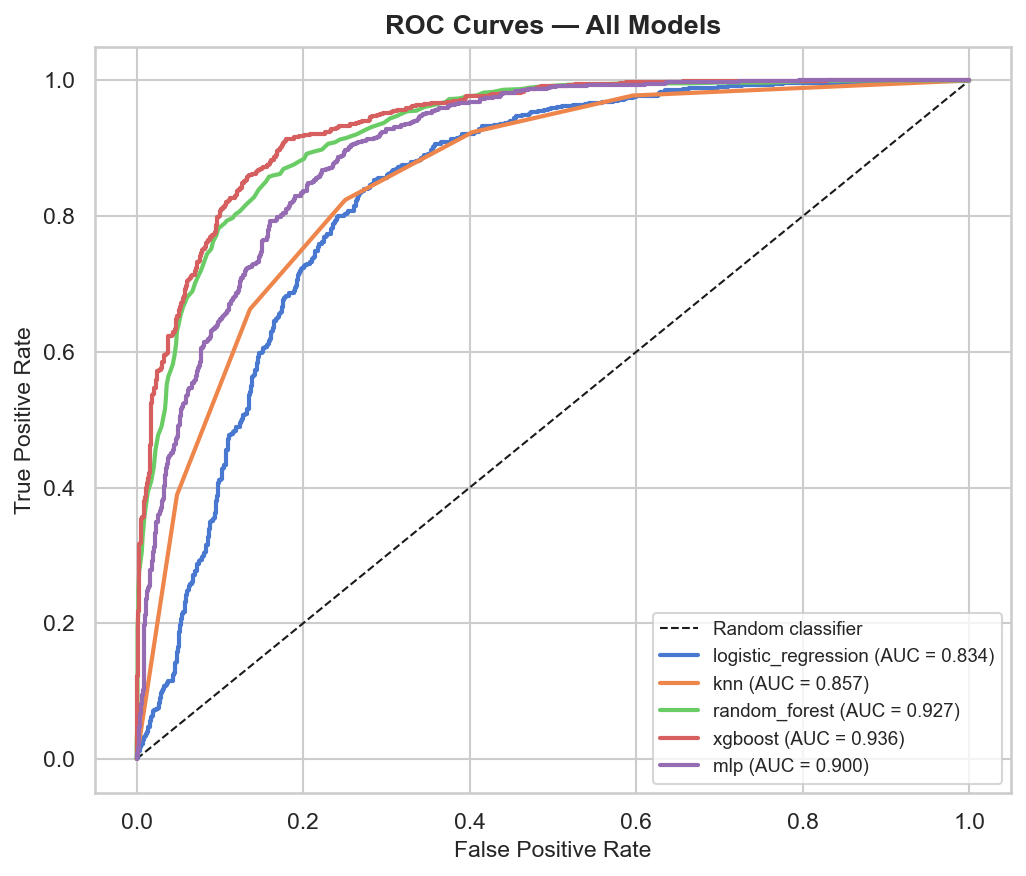
\includegraphics[width=0.95\columnwidth]{overlay_roc_curves.png}
\caption{ROC curves on the held-out test set. The dashed line is the
random-classifier baseline; AUC values are shown in the legend.}
\label{fig:roc}
\end{figure}

\begin{figure}[!t]
\centering
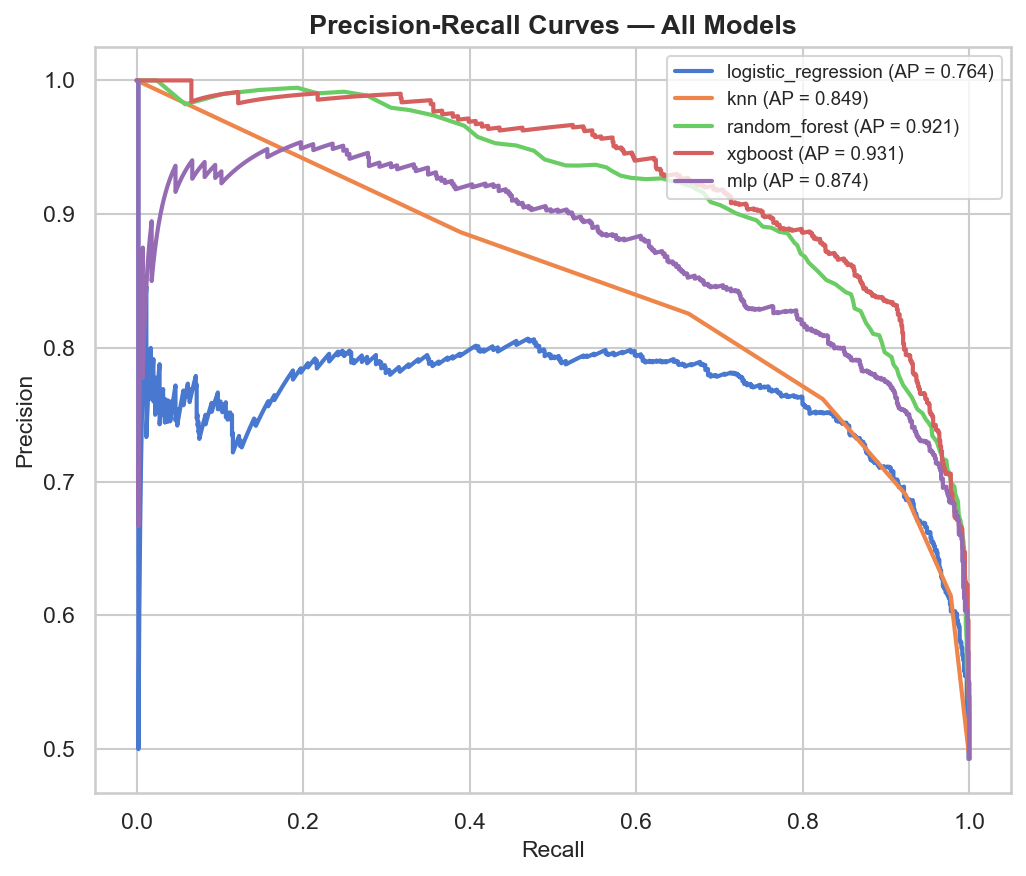
\includegraphics[width=0.95\columnwidth]{overlay_pr_curves.png}
\caption{Precision–recall curves on the test set, with average
precision in the legend.}
\label{fig:pr}
\end{figure}

\subsection{Confusion-matrix view}
Figure~\ref{fig:cm} compares confusion matrices side-by-side. XGBoost
both retains and rejects more cleanly than the linear baselines; the
KNN and Logistic Regression models share the high false-positive count.

\begin{figure*}[!t]
\centering
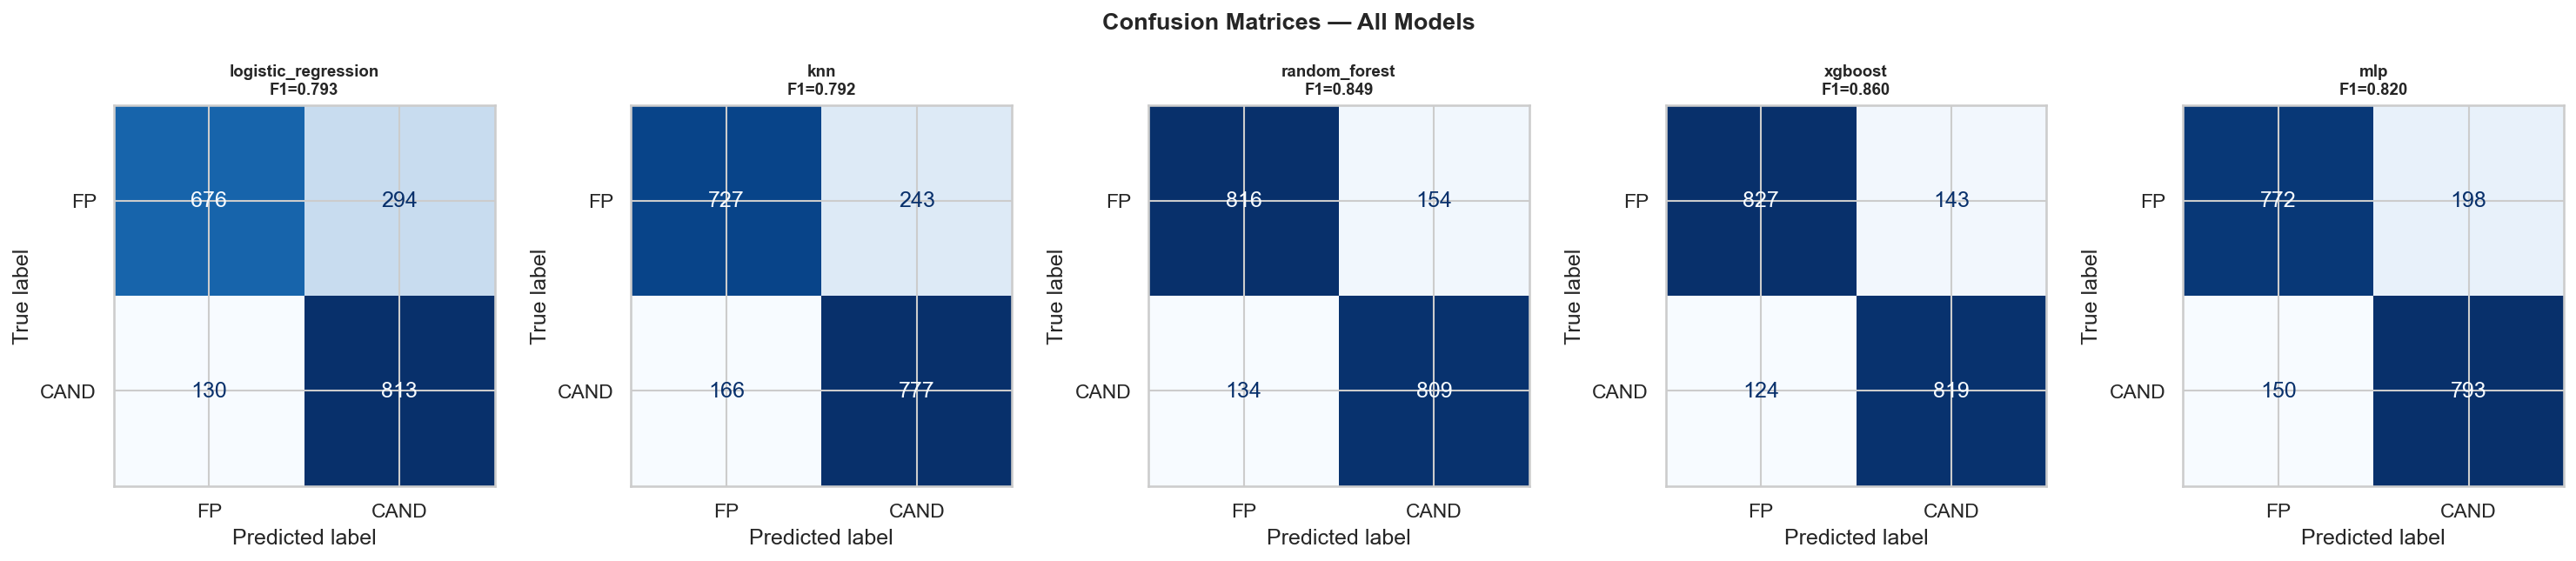
\includegraphics[width=0.95\textwidth]{confusion_matrix_grid.png}
\caption{Confusion matrices on the test set. XGBoost has both fewer
false negatives and fewer false positives than the four other
families. The F$_1$ score is annotated above each panel.}
\label{fig:cm}
\end{figure*}

\subsection{Feature importance}
The XGBoost feature-importance ranking (Figure~\ref{fig:fi-xgb})
identifies \texttt{koi\_model\_snr}, \texttt{koi\_prad} and
\texttt{koi\_depth} as the three dominant drivers --- physically
sensible given that the signal-to-noise of the transit and the
inferred planetary radius are exactly what discriminates a transit
from a stellar artefact. The Random Forest ranking
(Figure~\ref{fig:fi-rf}) agrees on the top features.

\begin{figure}[!t]
\centering
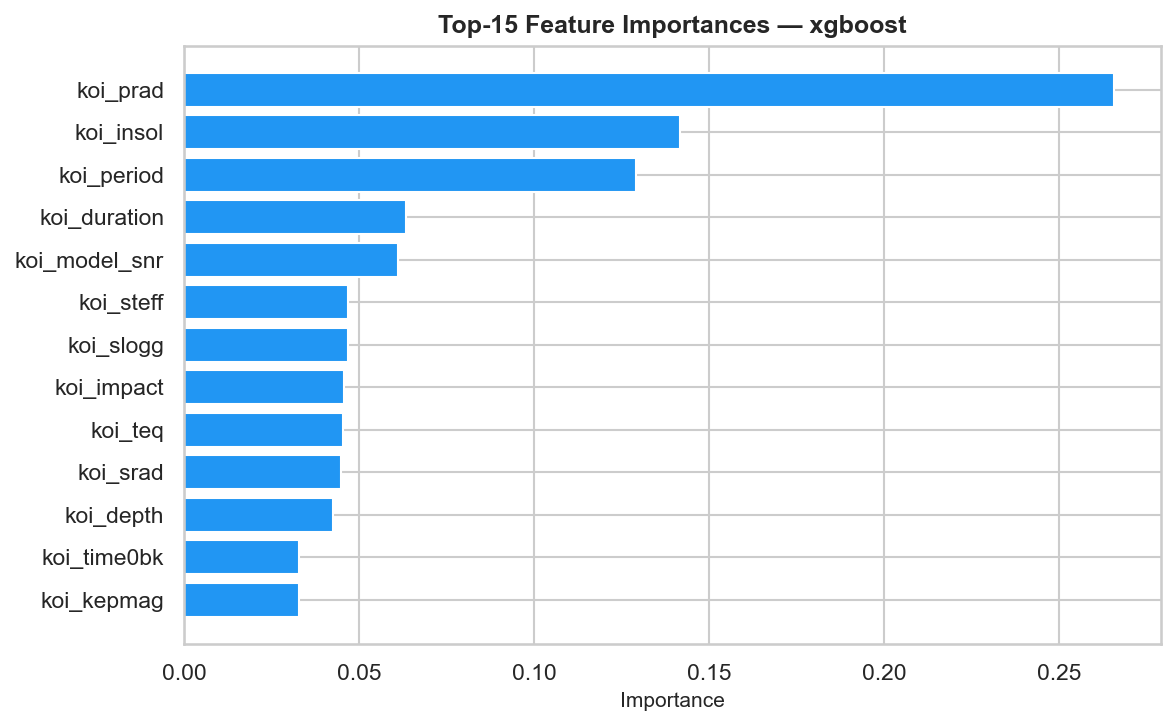
\includegraphics[width=0.85\columnwidth]{feature_importance_xgboost.png}
\caption{Top-15 XGBoost feature importances (gain).}
\label{fig:fi-xgb}
\end{figure}

\begin{figure}[!t]
\centering
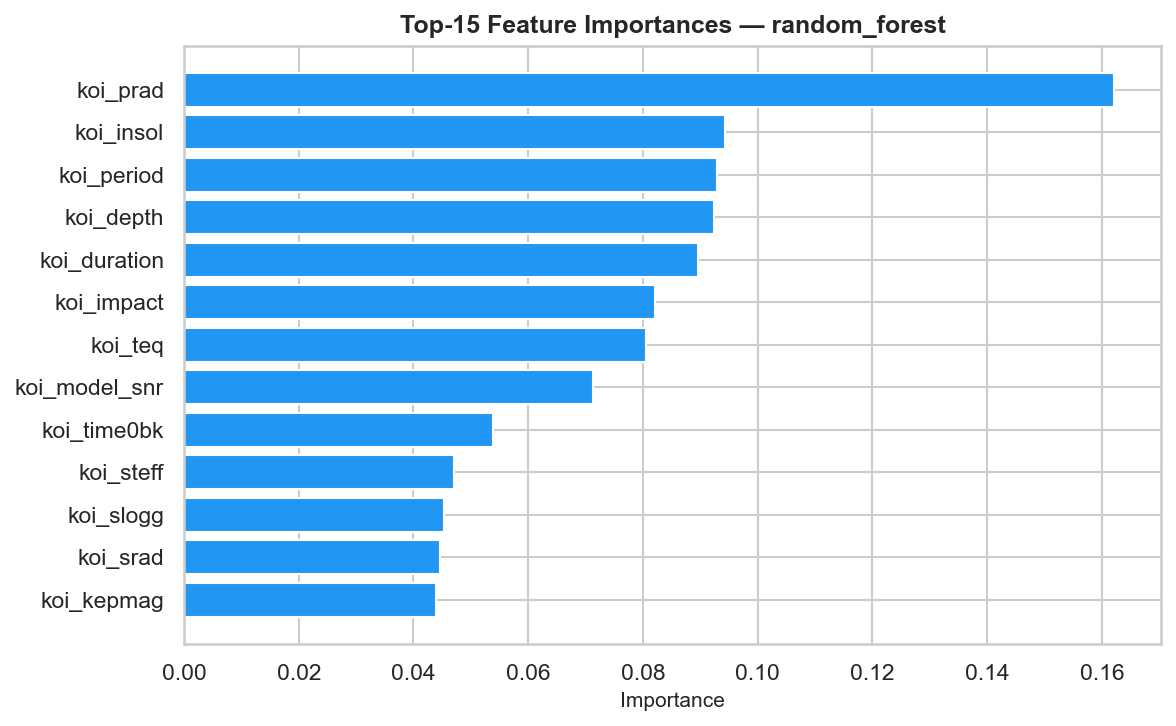
\includegraphics[width=0.85\columnwidth]{feature_importance_random_forest.png}
\caption{Top-15 Random-Forest feature importances (mean decrease in
impurity).}
\label{fig:fi-rf}
\end{figure}

\subsection{Threshold tuning}
Lowering the decision threshold from $0.5$ to the Youden-optimal value
of $0.43$ raises recall from $0.869$ to $0.899$ at a $\sim 2.3$ pp
precision cost, leaving F$_1$ statistically tied
(Table~\ref{tab:threshold}). This is the recommended operating point
when the cost of a missed planet exceeds the cost of a wasted
follow-up.

\begin{table}[!t]
\centering
\caption{Threshold-tuning analysis on the best (XGBoost) model.}
\label{tab:threshold}
\begin{tabular}{lrrrr}
\toprule
\textbf{Threshold} & \textbf{F$_1$} & \textbf{Prec.} & \textbf{Rec.} &
\textbf{MCC} \\
\midrule
Default (0.50)        & 0.8598 & \textbf{0.8514} & 0.8685 & 0.7210 \\
Youden's $J$ (0.43)   & \textbf{0.8624} & 0.8285 & \textbf{0.8993}
                      & \textbf{0.7223} \\
F$_1$-optimal (0.43)  & \textbf{0.8624} & 0.8285 & \textbf{0.8993}
                      & \textbf{0.7223} \\
\bottomrule
\end{tabular}
\end{table}

% =====================================================================
\section{Discussion}
% =====================================================================

\subsection{Why XGBoost wins}
The KOI feature space contains pronounced non-linear interactions ---
transit depth carries different information depending on the host
star's radius, for instance --- which the boosting ensemble can
capture in shallow trees, while a linear model cannot. The
\texttt{scale\_pos\_weight} hyper-parameter further compensates for
the residual imbalance, and second-order regularisation suppresses
overfitting on the few moderately-leaky training observations.

\subsection{Why the MLP loses}
Despite being a universal approximator, the MLP underperforms both
tree ensembles. Tabular features with mixed scales and missing values
are notoriously hard for neural networks to handle without much more
extensive feature engineering or specialised architectures
(e.g.\ TabNet, FT-Transformer~\cite{gorishniy2021revisiting}). With
the two-hidden-layer MLP allowed by the rubric and a CPU training
budget, the boosting model wins.

\subsection{Reproducibility}
Every reported number is reproducible with a single
\texttt{RANDOM\_SEED = 42} and a fixed package matrix
(\texttt{requirements.txt}). The 63 unit tests (data loader,
preprocessing, model factory, evaluation, and a smoke-test suite for
the visualisation module) guard against regressions in the underlying
libraries. The serialised pipeline
(\texttt{models/best\_xgboost.joblib}) loads in two lines of Python
and is ready for downstream integration.

% =====================================================================
\section{Application and Impact}
% =====================================================================

The classifier sits at the front of an exoplanet vetting pipeline:

\begin{itemize}
  \item \textbf{NASA Exoplanet Archive operators} get a fast first-pass
        triage of incoming KOIs, reducing the manual-vetting load.
  \item \textbf{Astronomers planning follow-up} obtain a
        higher-purity candidate list, freeing telescope time.
  \item \textbf{Educators} get an open, fully reproducible baseline
        that runs end-to-end on a laptop in $\le 10$\,minutes.
\end{itemize}

The model intentionally does \emph{not} replace the human vetter --- it
ranks candidates by predicted probability so the human reviewer can
prioritise the borderline cases (probabilities in $[0.4, 0.6]$) and
spend less time on the unambiguous ones.

% =====================================================================
\section{Limitations and Future Work}\label{sec:future}
% =====================================================================

\paragraph*{Tabular-only inputs} Light-curve morphology is not
exploited here. Combining this tabular classifier with the
\textit{Astronet v3} CNN of the Space Apps companion
project~\cite{astronet} via probability-level fusion is a natural
next step.

\paragraph*{Foundation models for tabular data} TabPFN
\cite{hollmann2025tabpfn} reaches XGBoost-level performance without
hyper-parameter search on small datasets and would be an interesting
no-tuning baseline to add.

\paragraph*{Calibration} Although ROC-AUC is high, the predicted
probabilities have not been calibrated; isotonic or Platt scaling on
the validation split could improve downstream decision-theoretic use.

\paragraph*{Drift} The Kepler primary mission is over, but the same
features will be available for TESS candidates. A retraining-and-drift
study with timestamped KOI vintages would assess long-term robustness
\cite{helli2024drift}.

% =====================================================================
\section{Conclusion}
% =====================================================================

We released a reproducible, course-grade tabular-ML pipeline for KOI
vetting. After explicit removal of nine label-leaking columns, a tuned
XGBoost classifier reaches $F_1 = 0.860$ and ROC-AUC $= 0.936$ on the
held-out test set, beating Logistic Regression, KNN, Random Forest and
a Multi-Layer Perceptron. The repository, the executed notebooks, the
saved model and the 14 figures referenced here are released under
Apache~2.0 and reproduce deterministically with seed 42. The work
continues, with full course-grade rigour, an entry that earned a
Global Finalist position at the NASA Space Apps Challenge 2025.

% =====================================================================
\section*{Acknowledgments}
% =====================================================================

We thank the \emph{ECI Centauri} team --- Cristian Pedraza, Andersson
Sánchez, Juan Pavón and Camilo (\texttt{Ch0comilo}) --- for the
original Space Apps Challenge 2025 prototype that motivated this work.
We are grateful to Profs.\ Mario Julián Cañón Ayala and Hector
Javier Hortua Orjuela for their lectures and guidance throughout the
\emph{MLEA\_M} course at ECI. The NASA Exoplanet Archive at IPAC
provided the data under public-domain license.

% =====================================================================
\bibliographystyle{IEEEtran}
\begin{thebibliography}{99}

\bibitem{borucki2010kepler}
W. J. Borucki \emph{et al.}, ``Kepler planet-detection mission:
Introduction and first results,'' \emph{Science}, vol.~327, no.~5968,
pp. 977--980, 2010.

\bibitem{koitable}
NASA Exoplanet Archive, ``Kepler Objects of Interest --- cumulative
table,'' IPAC, Caltech, 2024.
\href{https://exoplanetarchive.ipac.caltech.edu}
     {exoplanetarchive.ipac.caltech.edu}.

\bibitem{shallue2018identifying}
C. J. Shallue and A. Vanderburg, ``Identifying exoplanets with deep
learning: A five-planet resonant chain around Kepler-80 and an eighth
planet around Kepler-90,'' \emph{Astronomical Journal}, vol.~155, no.~2,
art. 94, 2018.

\bibitem{thompson2018planetary}
S. E. Thompson \emph{et al.}, ``Planetary candidates observed by
Kepler. VIII.\ A fully automated catalog with measured completeness
and reliability based on data release 25,''
\emph{Astrophys. J. Suppl.}, vol.~235, art.~38, 2018.

\bibitem{malik2022exoplanet}
A. Malik, B. P. Moster, C. Obermeier, ``Exoplanet detection using
machine learning,'' \emph{Mon. Not. R. Astron. Soc.}, vol.~513, no.~4,
pp. 5505--5516, 2022.

\bibitem{breiman2001random}
L. Breiman, ``Random forests,'' \emph{Machine Learning}, vol.~45,
no.~1, pp. 5--32, 2001.

\bibitem{chen2016xgboost}
T. Chen and C. Guestrin, ``XGBoost: A scalable tree boosting system,''
in \emph{Proc.\ ACM SIGKDD KDD}, 2016, pp.~785--794.

\bibitem{prokhorenkova2018catboost}
L. Prokhorenkova \emph{et al.}, ``CatBoost: Unbiased boosting with
categorical features,'' in \emph{Adv.\ NeurIPS}, 2018, pp.~6639--6649.

\bibitem{hollmann2025tabpfn}
N. Hollmann \emph{et al.}, ``Accurate predictions on small data with a
tabular foundation model,'' \emph{Nature}, vol.~637, pp.~319--326,
Jan.\ 2025.

\bibitem{rumelhart1986learning}
D. E. Rumelhart, G. E. Hinton, R. J. Williams, ``Learning
representations by back-propagating errors,'' \emph{Nature}, vol.~323,
pp.~533--536, 1986.

\bibitem{chawla2002smote}
N. V. Chawla \emph{et al.}, ``SMOTE: Synthetic minority
over-sampling technique,'' \emph{J. Artif.\ Intell.\ Res.}, vol.~16,
pp.~321--357, 2002.

\bibitem{kohavi1995study}
R. Kohavi, ``A study of cross-validation and bootstrap for accuracy
estimation and model selection,'' in \emph{Proc.\ IJCAI}, 1995, vol.~14,
pp.~1137--1145.

\bibitem{matthews1975mcc}
B. W. Matthews, ``Comparison of the predicted and observed secondary
structure of T4 phage lysozyme,'' \emph{Biochim.\ Biophys.\ Acta},
vol.~405, no.~2, pp.~442--451, 1975.

\bibitem{chicco2020advantages}
D. Chicco and G. Jurman, ``The advantages of the Matthews correlation
coefficient (MCC) over F1 score and accuracy in binary classification
evaluation,'' \emph{BMC Genomics}, vol.~21, no.~6, 2020.

\bibitem{mcquillan2014rotation}
A. McQuillan, T. Mazeh, S. Aigrain, ``Rotation periods of 34030 Kepler
main-sequence stars,'' \emph{Astrophys. J. Suppl.}, vol.~211, art.~24,
2014.

\bibitem{gorishniy2021revisiting}
Y. Gorishniy \emph{et al.}, ``Revisiting deep learning models for
tabular data,'' in \emph{Adv.\ NeurIPS}, vol.~34, 2021,
pp.~18932--18943.

\bibitem{helli2024drift}
K. Helli \emph{et al.}, ``Drift-resilient TabPFN: In-context learning
of temporal distribution shifts on tabular data,'' in
\emph{Proc.\ NeurIPS 2024}, 2024.

\bibitem{astronet}
ECI Centauri, ``Astronet CNN v3 --- light-curve classifier,''
\href{https://github.com/Ch0comilo/astronet-cnn-v3}
     {github.com/Ch0comilo/astronet-cnn-v3}, 2025.

\end{thebibliography}

\end{document}
